\documentclass[letterpaper,11pt,notitlepage]{article}
% define the title
\usepackage{amsmath}
\usepackage{fixltx2e}
\usepackage{graphicx}
\usepackage[labelformat=empty]{caption}
\usepackage{subcaption}
\usepackage{listings}
\usepackage{color}
\usepackage{relsize}
\usepackage{wrapfig}
\usepackage{fontspec}
\usepackage{hyperref}
\usepackage{hanging}
\usepackage{textcomp,    % for \textlangle and \textrangle macros
            xspace}
\newcommand\la{\textlangle}  % set up short-form macros
\newcommand\ra{\textrangle\xspace}
\newcommand\rans{\textrangle}
\lstset{
  language={matlab},
  basicstyle=\ttfamily\smaller\relax,	
  tabsize=4,                              % Default tab size
  % showspaces=false,                       % Dont make spaces visible
  showtabs=false,                         % Dont make tabls visible
  columns=flexible,                       % Column formatc
  commentstyle=\color{mygreen}\textit,           % comment style
  extendedchars=true,              % lets you use non-ASCII characters; for 8-bits encodings only, does not work with UTF-8
  numbers=left,                    % where to put the line-numbers; possible values are (none, left, right)
  numbersep=8pt,                   % how far the line-numbers are from the code
  numberstyle=\tiny\color{mygray}, % the style that is used for the line-numbers
  stepnumber=1,
  xleftmargin=2cm,
  % backgroundcolor=\color{light-gray},
  breaklines=true,
  keywordstyle=\color{mynavy}
}
\hypersetup{colorlinks=true,linkcolor=blue}
\renewcommand*{\UrlFont}{\ttfamily\smaller\relax}

% \addtolength{\oddsidemargin}{0.5in}
% \addtolength{\evensidemargin}{0.5in}
% \addtolength{\textwidth}{-1in}
\addtolength{\topmargin}{-1in}
\addtolength{\textheight}{1.75in}
\setlength\parindent{24pt}

\definecolor{mygreen}{rgb}{0.1020,0.5961,0.3137}
\definecolor{mygray}{rgb}{0.5,0.5,0.5}
\definecolor{light-gray}{rgb}{0.8,0.8,0.8}
\definecolor{mynavy}{rgb}{0.1922,0.2118,0.5843}

\begin{document}

\begin{center}
	Homework 4 - LEARNABILITY\\
	2015 Spring, Machine Learning\\
	Choong-Wan Woo\\
	\today\\
\end{center}

\hspace*{-1cm}\textbf{Problem 2.3.}  \rule{10.5cm}{0.4pt}\\
\noindent\textit{Concentric circles.}\\

\indent With concentric circles as concepts, we can define one annulus error area, \textit{E} (see \textbf{Figure 1}), that has the probability of falling in this region, $\epsilon$. The annulus area, \textit{E}, can be defined as $E = \{(x,y):e^2\le x^2+y^2 \le r^2\}$, with $e = \inf\{e:\Pr[\pi(r^2-e^2)]\ge \epsilon\}$\\
\indent By contraposition, if $R(\text{R}_S)>\epsilon$ (here, $R(\text{R}_S)$ denotes \textit{the expected error of} $\text{R}_S$), then $\text{R}_S$ must miss the error region \textit{E}. As a result, we can write
\begin{align*}
\Pr [R(\text{R}_S)>\epsilon] &\le \Pr[\{\text{R}_S\cap E =\emptyset\}]\\
&\le(1-\epsilon)^m\\
&\le e^{-\epsilon m}
\end{align*}
\noindent For any $\delta >0$, to ensure that $\Pr[R(\text{R}_S) > \epsilon] \le \delta$, we can impose
\[e^{-\epsilon m} \le \delta\]
If we solve this in terms of \textit{m}, we get
\[m \ge \frac{1}{\epsilon}\log \frac{1}{\delta}\]
\noindent Thus, for any $\epsilon >0, \delta>0$, if the sample size \textit{m} is greater than $\frac{1}{\epsilon}\log \frac{1}{\delta}$, then $\Pr[R(\text{R}_S) > \epsilon] \le \delta$. Therefore, this class can be $(\epsilon,\delta)$-PAC-learnable from training data size $m \ge \frac{1}{\epsilon}\log \frac{1}{\delta}$

\begin{figure}[ht!]
	\centering
	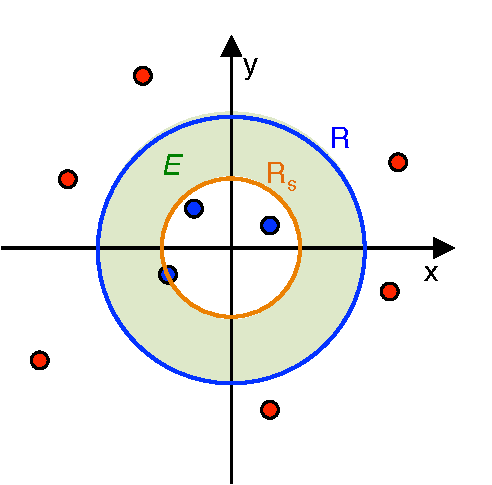
\includegraphics[width=6cm]{Figure1}
	\captionsetup{width=.8\textwidth}
	\caption{\textbf{Figure 1.} Illustration of the concentric circle case.} 
\end{figure} \leavevmode \\

\hspace*{-1cm}\textbf{Problem 2.4.}  \rule{10.5cm}{0.4pt}\\
\noindent\textit{Non-concentric circles. Can you tell Gertrude if her approach works?}\\

\indent Gertrude's approach will not work because her approach relies on wrong assumptions. Most importantly, with non-concentric circles, false positive errors can be made outside of a target concept, R, as demonstrated in \textbf{Figure 2}. Therefore, drawing three regions, $r_1, r_2, r_3,$ inside R and defining the regions in terms of $\epsilon$ is not useful, and certainly, those three regions, $r_1, r_2, r_3,$ do not have the equal probabilities of $\epsilon$/3.\\
\indent In addition, we can think of a counterexample of Gertrude's approach. As \textbf{Figure 2} shows, even though training data do not miss $r_1, r_2, r_3$ regions, it can still make the generalization error. Thus the equation from her approach 
$\Pr[R(\text{R}_S)>\epsilon]\le \Pr[\bigcup^{3}_{i=1}\{\text{R}_S \bigcap r_i=\emptyset\}]$, which is similar to the equation 2.5 of the textbook, should be wrong in this non-concentric circle case. 

\begin{figure}[ht!]
	\centering
	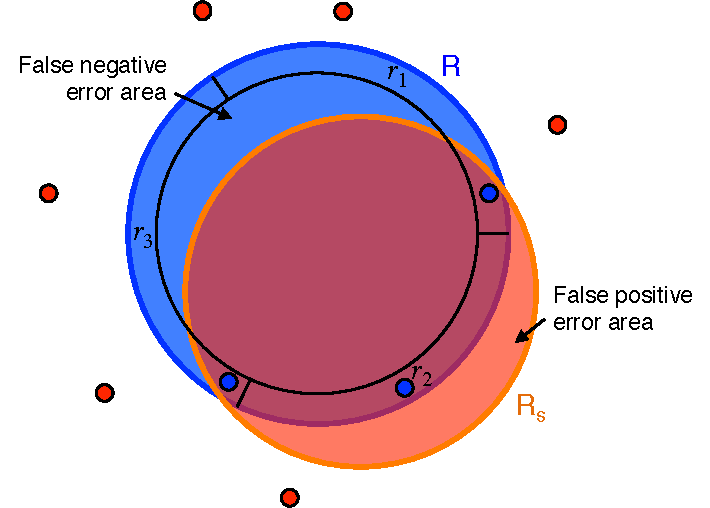
\includegraphics[width=7.5cm]{Figure2}
	\captionsetup{width=.8\textwidth}
	\caption{\textbf{Figure 2.} Illustration of the non-concentric circle case.} 
\end{figure} \leavevmode \\

\hspace*{-1cm}\textbf{Problem 2.6.}  \rule{10.5cm}{0.4pt}\\
\noindent\textit{Learning in the presence of noise-rectangles.}\\\\

\noindent (a) The probability that $\text{R}^\prime$ misses a region $r_j$ equals the sum of 1) the probability that 
no data in $\text{R}^\prime$ fall on a region $r_j$ and 2) the probability that the positive training point that fall on a region $r_j$ is flipped to negative with probability $\eta^\prime$. 
\begin{align*}
\Pr[\text{R}^\prime \text{ misses }r_j] &= \Pr[\{\text{R}^\prime \cap r_j =\emptyset\}] + \eta^\prime\Pr[\{\text{R}^\prime \cap r_j \neq\emptyset\}]\\
&= 1-\frac{\epsilon}{4} + \eta^\prime\times\frac{\epsilon}{4}\\
&= 1+\frac{(\eta^\prime-1)\epsilon}{4}\\
\end{align*}

\noindent (b) The upper bound on $\Pr[R(\text{R}^\prime)>\epsilon]$ can be derived as follows:
\begin{align*}
\Pr[R(\text{R}^\prime)>\epsilon] &\le \Pr_{S\sim D^m}[\bigcup^{4}_{i=1}\{\text{R}^\prime \text{ misses }r_j\}]\\
&\le \sum^{4}_{i=1} \Pr_{S\sim D^m}[\{\text{R}^\prime \text{ misses }r_j\}]\\
&\le 4(1+\frac{(\eta^\prime-1)\epsilon}{4})^m\\
&\le 4e^{(\eta^\prime-1)m\epsilon/4}\\
\end{align*}

\indent For any $\delta >0$, to ensure that $\Pr[R(\text{R}^\prime)>\epsilon] \le \delta$, we can impose
\[4e^{(\eta^\prime-1)m\epsilon/4} \le \delta\]
\indent, solving for \textit{m}:
\[m\ge\frac{4}{(1-\eta^\prime)\epsilon}\ln\frac{4}{\delta}\]\leavevmode \\

\hspace*{-1cm}\textbf{Problem 3.5.}  \rule{10.5cm}{0.4pt}\\
\noindent Consider the really simple hypotheses that always provide 1 or -1. Then, VC-dimension of the hypothesis set is 1 because the functions cannot shatter two points. In this case, Prof. Jesetoo's new bound becomes 
\[\Re_m(H) \le O(\frac{1}{m})\]
From eq. 3.31-3.32 on page 48 of the textbook, we know that 
\[\hat{\Re}_m(H) \le O\Big(\sqrt{\frac{\log m}{m}}\Big)\]
From eq. 3.14 on page 36 of the textbook, 
\begin{align*}
\Re_m(H) &\le \hat{\Re}_m(H)+\sqrt{\frac{\log \frac{2}{\delta}}{2m}}\\
&\le O\Big(\sqrt{\frac{\log m}{m}}\Big)
\end{align*}
With $m \ge 1, \sqrt{\frac{\log m}{m}}$ is always greater than $O(\frac{1}{m})$.\\\\

\hspace*{-1cm}\textbf{Problem 3.12.}  \rule{10.5cm}{0.4pt}\\
\noindent\textit{VC-dimension of sine functions.}\\

\noindent (a) To solve this problem, we need to think about the pattern of sine values of $x, 2x, 3x$, and $4x$. $\sin(2\omega x)$ has the twice larger frequency than $\sin(\omega x)$, $\sin(3\omega x)$ has the three times larger frequency than $\sin(\omega x)$, and $\sin(4\omega x)$ has the four-times larger frequency than $\sin(\omega x)$ and the twice larger frequency than $\sin(2\omega x)$. Therefore, the exact pattern of four sine values is repeated for $x$, as \textbf{Figure 3} shows (in \textbf{Figure 3}, \textit{the repetitive pattern in red} points out the pattern). \textbf{Figure 3} shows twelve possible combinations of signs of four points that can be shattered by sine functions. Given that there are 16 possible combinations of signs in four points ($2^4 = 16$), there are four sign combinations that cannot be shattered by the sine functions, including $(+,+,-,+), (-,-,+,-), (+,-,-,-),$ and $(-,+,+,+)$. Therefore, the points, $x, 2x, 3x$, and $4x$ cannot be shattered by this family of sine functions. 

\begin{figure}[ht!]
	\hspace*{-2cm}
	\centering
	\includegraphics[width=16cm]{Figure3_12_ela}
	\captionsetup{width=.8\textwidth}
	\caption{\textbf{Figure 3.} Point values (signs) that can be shattered by four sine functions ($\sin(\omega x), \sin(2\omega x), \sin(3\omega x), \sin(4\omega x)$). The maximum number of possible combinations of signs of four points is $2^4 = 16$, and the number of cases that can be shattered by sine functions are twelve. Therefore, there are four combinations that cannot be shattered by the family of sine functions.} 
\end{figure} \leavevmode \\

\noindent (b)\\
According to the hint, consider $x_i = 2^{-i}$ for $i \le m$. If we can find the correct parameter $\omega$ that is the function of $y_i$, such that $\omega x_i$ yields the values between $-\pi<\omega x_i<0$ or $\pi<\omega x_i<2\pi$ when $y_i=-1$, and the values between $0<\omega x_i<\pi$ when $y_i=+1$. This was my approach to this problem, but it was difficult to find the right $\omega$ value.\\\\

\hspace*{-1cm}\textbf{Problem 3.13. (or 3.6 in the new version of textbook)}  \rule{2.5cm}{0.4pt}\\
\noindent\textit{VC-dimension of the union of k intervals.}\\

\noindent The answer is 2\textit{k}. The union of \textit{k} intervals can shatter 2\textit{k} points in one the real line, as \textbf{Figure 4a} suggests. In \textbf{Figure 4a}, I showed the most complicated case using 2\textit{k} points (where $+1$ and $-1$ alternates) and how the union of \textit{k} intervals can shatter it. Then, we can add one additional $+1$ point after the last point of 2\textit{k} points. The $(2k+1)$-th point cannot be shattered with \textit{k} intervals, as \textbf{Figure 4b} suggested. Therefore, the VC-dimension of the union of \textit{k} intervals is 2\textit{k}.

\begin{figure}[ht!]
	\centering
	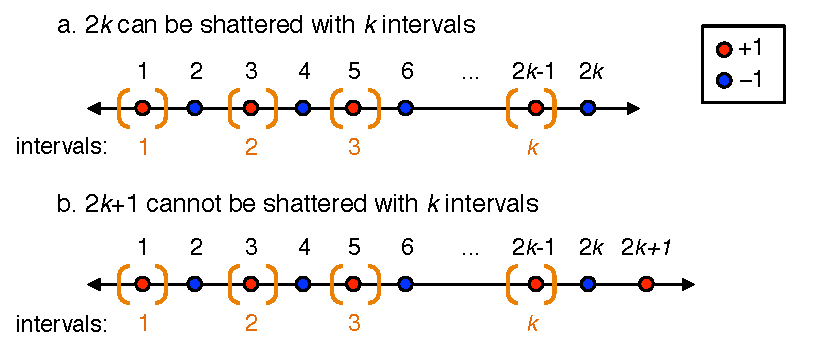
\includegraphics[width=11cm]{Figure3_13}
	\captionsetup{width=.8\textwidth}
	\caption{\textbf{Figure 4.} VC-dimensions of the union of \textit{k} intervals.} 
\end{figure}

\hspace*{-1cm}\textbf{Problem 3.19.}  \rule{10.5cm}{0.4pt}\\
\noindent\textit{Biased coins.}\\

\noindent (a)
\begin{align*} 
error(f_o) &= \Pr [f_o(S) \neq x]\\
&= \Pr[f_o(S)=x_A|x=x_B]\Pr[x=x_B]+\Pr[f_o(S)=x_B|x=x_A]\Pr[x=x_A]\\ 
\end{align*}
where $\Pr[x=x_A]=\Pr[x=x_B]=1/2$. Therefore,\\
\begin{align*} 
&= \frac{1}{2}\Pr[f_o(S)=x_A|x=x_B]+\frac{1}{2}\Pr[f_o(S)=x_B|x=x_A]\\ 
\end{align*}
where $f_o(S)=x_A$ is same with $N(S)<m/2$, and $f_o(S)=x_B$ is same with $N(S)\ge m/2$ by definition. Therefore,\\
\begin{align*} 
&= \frac{1}{2}\Pr[N(S)<\frac{m}{2}|x=x_B]+\frac{1}{2}\Pr[N(S)\ge\frac{m}{2}|x=x_A]\\
&\ge \frac{1}{2}\Pr[N(S)\ge\frac{m}{2}|x=x_A]\\ 
\end{align*}

\noindent (b)\\
Tossing a coin ($x_A$) follows a binomial distribution with $p = (1-\epsilon)/2$. Slud's inequality (D.3.1) on page 374 of the textbook says, if $p \le 1/2$ and $mp \le k \le m(1-p)$,
\[\Pr[B\ge k] \ge \Pr[N\ge \frac{k-mp}{\sqrt{mp(1-p)}}]\]
$\frac{1}{2}\Pr[N(S)\ge\frac{m}{2}|x=x_A]$ in (a) can be formulated as $B(m,p) \ge k$, where $k = m/2$ and $p = (1-\epsilon)/2$. Therefore, 
\begin{align*} 
error(f_o) &\ge \frac{1}{2}\Pr[N(S)\ge\frac{m}{2}|x=x_A]\\ 
&\ge \frac{1}{2}\Pr[N \ge \frac{\frac{m}{2}-m(\frac{1-\epsilon}{2})}{\sqrt{m(\frac{1-\epsilon}{2})(\frac{1+\epsilon}{2})}}]\\
&= \frac{1}{2}\Pr[N \ge \frac{m\epsilon/2}{\sqrt{m(1-\epsilon^2)/4}}]\\
&= \frac{1}{2}\Pr[N \ge \frac{\sqrt{m}\epsilon}{\sqrt{1-\epsilon^2}}]
\end{align*} 
According D.3.2. on page 374 of the textbook, if \textit{N} is a random variable following the normal distribution, then for $u > 0$,
\[\Pr[N \ge u] \ge \frac{1}{2}(1-\sqrt{1-e^{-u^2}})\]
From the previous equation, we can consider $u = \frac{\sqrt{m}\epsilon}{\sqrt{1-\epsilon^2}}$. Then, 
\[error(f_o) \ge \frac{1}{4}(1-\sqrt{1-e^{-\frac{m\epsilon^2}{1-\epsilon^2}}})\]\\

\noindent (c)\\
If \textit{m} is odd, we can use $k = (m+1)/2$ instead of $k=m/2$ in the probability expression. Therefore, $\Pr[N(S)\ge \frac{m}{2}|x=x_A]$ becomes $\Pr[N(S)\ge \frac{m+1}{2}|x=x_A]$. For both cases, we can use the following expression,
\[\Pr[N(S)\ge \lceil\frac{m}{2}\rceil|x=x_A]\]
Therefore, we can replace $m/2$ in previous equation with $\lceil m/2 \rceil$:
\[error(f_o) \ge \frac{1}{4}(1-\sqrt{1-e^{-\frac{2\lceil m/2 \rceil \epsilon^2}{1-\epsilon^2}}})\]\\

\noindent (d)\\
Oskar's error is at most $\delta$,
\[\frac{1}{4}(1-\sqrt{1-e^{-\frac{2\lceil m/2 \rceil \epsilon^2}{1-\epsilon^2}}}) < \delta\]
\[\Longrightarrow 1-\sqrt{1-e^{-\frac{2\lceil m/2 \rceil \epsilon^2}{1-\epsilon^2}}} < 4\delta\]
\[\Longrightarrow \sqrt{1-e^{-\frac{2\lceil m/2 \rceil \epsilon^2}{1-\epsilon^2}}} > 1-4\delta\]
\[\Longrightarrow 1-e^{-\frac{2\lceil m/2 \rceil \epsilon^2}{1-\epsilon^2}} > (1-4\delta)^2\]
\begin{align*} 
\Longrightarrow e^{-\frac{2\lceil m/2 \rceil \epsilon^2}{1-\epsilon^2}} &< 1-(1-4\delta)^2\\
&=1-1+8\delta-16\delta^2\\
&=8\delta(1-2\delta)
\end{align*} 
\[\Longrightarrow \frac{-2\lceil m/2 \rceil \epsilon^2}{1-\epsilon^2}<\ln(8\delta(1-2\delta))\]
\[\Longrightarrow \lceil m/2 \rceil > \frac{1-\epsilon^2}{2\epsilon^2}\ln(8\delta(1-2\delta))\]
\[\Longrightarrow m > 2\lceil \frac{1-\epsilon^2}{2\epsilon^2} \rceil \ln(8\delta(1-2\delta))\]

\noindent (e)\\
Couldn't solve this. 

\end{document}